\subsection{Entity Stats}
Entities in Head (E_{head}): 8949
Entities in Tail (E_{tail}): 379342
Total Count of entities in Head : 6562784
Total Count of entities in Tail : 9764565
 

Tail queries have been often mapped to the head \cite{} by using bag-of-word representations.
Lately they have also been linked with the head queries through entities. However, in this work
we attempt to quantify the extent to which the entities in the tail can be linked to entities 
in the head queries. It is important to know how much will entity linking at tail benefit query mining. 
We shall, from now on refer to entities in head queries as `head entity' 
and entities occuring in the tail as `tail entity'. 

%1.no of queries with head and tail ent
%2.Head and tail entity histogram for queries with more than 1 ent 
We begin by analyzing the volume of entities found in the tail. Of X unique tail queries,
63.2\% contain atleast one entity. Of queries containing more than one entity,  
86.2\% queries contain atleast one head entity. Table \ref{table:entDist} shows the number of 
queries, corresponding number of entities and the head to tail entity ratio in query. 
Head to Tail entity ratio is calculated by dividing number of head entities with number of 
tail entities in the query. The table clearly shows that for every tail entity there is a 
head entity in the query. Although, there are queries with more than 6 entities, 
they are too few to draw any significant conclusions. 
\begin{table}
\caption{\#Entities vs \#Queries}
\label{table:entDist}
\centering
\begin{tabular}{|l|l|l|}
\hline
\#Entities & \#Queries & Head Tail Ratio \\ \hline
1 & 2622873 & NA \\ \hline
2 & 1731256 & 0.48 \\ \hline
3 & 457946  & 0.91 \\ \hline
4 & 74125 & 1.09  \\ \hline
5 & 10757 & 1.07 \\ \hline
6 & 2416  & 0.97 \\ \hline
\end{tabular}
\end{table}

Figure \ref{img:headTailEntBreakup} shows the number of queries for each ratio. 
WRITE MORE ABOUT THE PLOT

\begin{figure}[t]
\label{img:headTailEntBreakup}
\caption{\%Queries vs Head to Tail Entity Ratio}
  \centering
    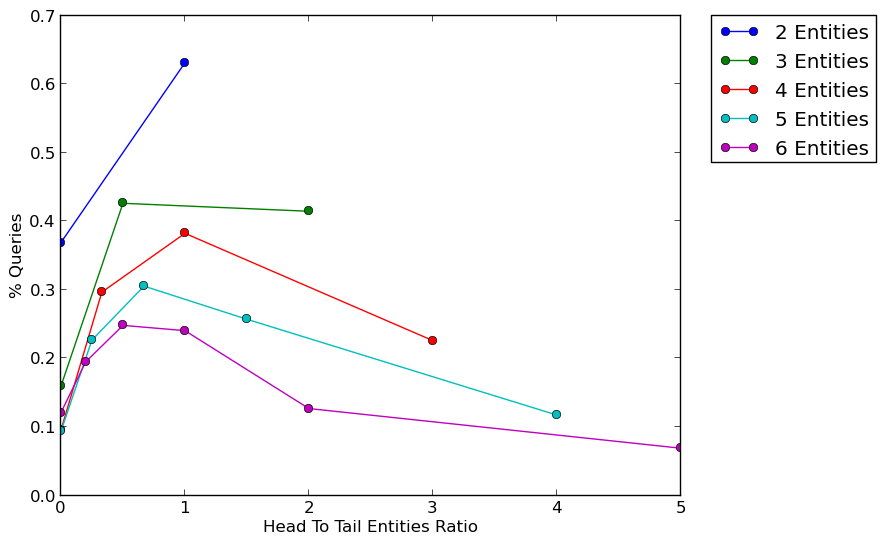
\includegraphics[width = 0.45\textwidth]{images/entity-head-query-ratio-dist.png}
\end{figure}

%Head entity popularity
Given that there would several head entities, not all of them will be equally popular. 
Here, popularity of the entity refers to the scope of that entity, how many entities does 
it co-occur with, or how common is that entity. 
Figure \ref{img:headEntDist} shows the frequency distribution of head entities in the 
head queries. That is, how frequently does a head entity occur in popular queries. 
To aggregate statistics for the tail, we divide head entities into 7 buckets, each bucket
spanning 20\% of entities. This results in X popular entities being in 0-20\% range, Y 
entities in 20-40\% range, so on and so forth. 


\begin{figure}[t]
\label{img:headEntDist}
\caption{Cumulative Distribution of Entity Frequency in Head Queries}
  \centering
    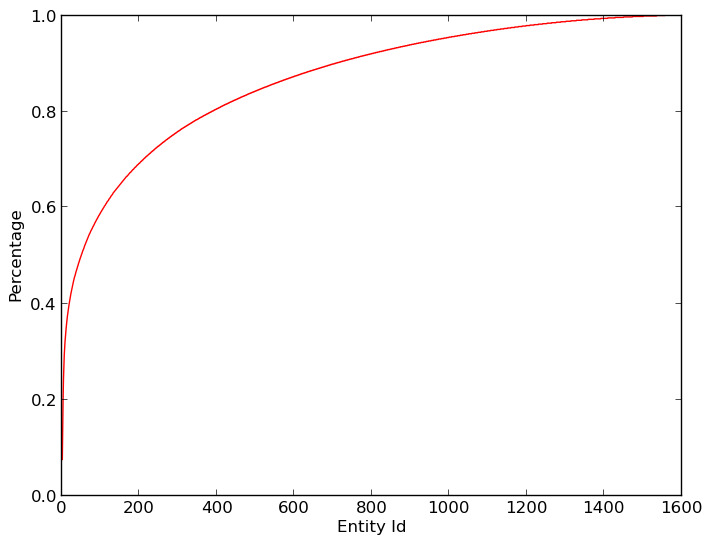
\includegraphics[width = 0.45\textwidth]{images/entity-head-dist.png}
\end{figure}



The co-occurrance of tail entities with head entities of different grades is shown in 
Figure \ref{img:headEntDistInTail}. The figure clearly indicates that 
WRITE ABOUT THE PLOT HERE

 
\begin{table}
\caption{Queries per Popularity of Head Entity}
\label{table:headEntQueryDist}
\centering
\begin{tabular}{|l|l|l|}
\hline
Popularity & \#Entities & Queries \\ \hline
0-20\% & 3 & 14851 \\ \hline
20-40\% & 18  & 57611.0 \\ \hline
40-60\% & 95 & 149733.0 \\ \hline
60-80\% & 287 & 299561.0 \\ \hline
80-95\% & 560 & 569271.0 \\ \hline
95-97\% & 236 & 298498.0 \\ \hline
97-100\% & 349 & 854345. 0  \\ \hline
\end{tabular}
\end{table}


\begin{figure}[t]
\label{img:headRankInTail}
\caption{\%Queries vs Rank of Head Entities}
  \centering
    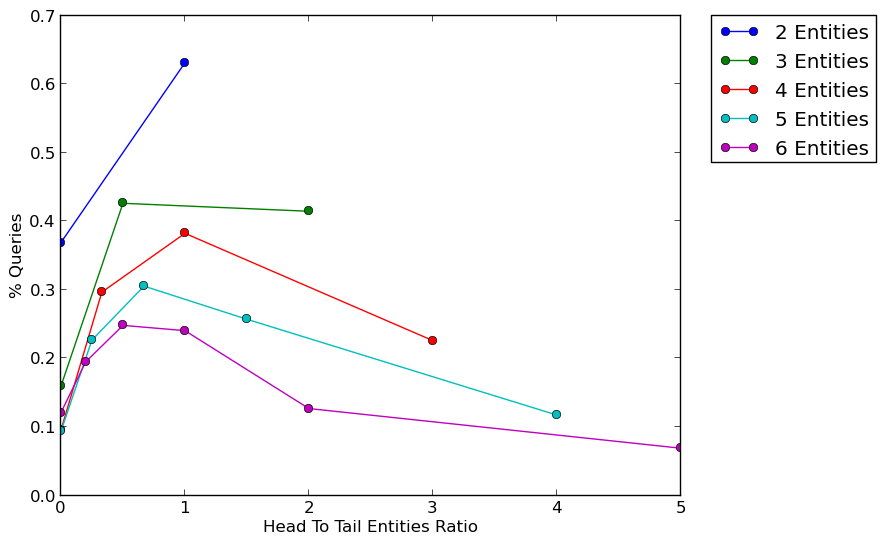
\includegraphics[width = 0.45\textwidth]{images/entity-head-query-ratio-dist.png}
\end{figure}

%In entity analysis of Aol query logs we calculate the following:
%\begin{itemize}
%\item No of queries with entities from the head or tail
%\item Frequency distribution of entities in head and tail
%\item Head and tail entity distribution in queries
%\end{itemize}




